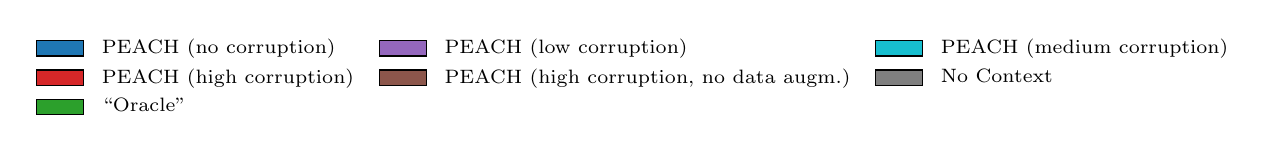
\begin{tikzpicture}
    \tikzstyle{every node}=[font=\scriptsize]
    \definecolor{tabblue}{RGB}{31, 119, 180}
\definecolor{taborange}{RGB}{255, 127, 14}
\definecolor{tabgreen}{RGB}{44, 160, 44}
\definecolor{tabred}{RGB}{214, 39, 40}
\definecolor{tabpurple}{RGB}{148, 103, 189}
\definecolor{tabbrown}{RGB}{140, 86, 75}
\definecolor{tabpink}{RGB}{227, 119, 194}
\definecolor{tabgray}{RGB}{127, 127, 127}
\definecolor{tabolive}{RGB}{188, 189, 34}
\definecolor{tabcyan}{RGB}{23, 190, 207}
\definecolor{ForestGreen}{RGB}{34, 139, 34}

    \begin{axis}[%
        hide axis,
        xmin=10,
        xmax=50,
        ymin=0,
        ymax=0.1,
        legend style={
            draw=none,
            legend cell align=left,
            legend columns=3,
            /tikz/every odd column/.append style={column sep=1ex},
            /tikz/every even column/.append style={column sep=1.6ex},
        }
    ]

        \addlegendimage{area legend, fill=tabblue}
    \addlegendentry{PEACH (no corruption)}

    \addlegendimage{area legend, fill=tabpurple}
    \addlegendentry{PEACH (low corruption)}

    \addlegendimage{area legend, fill=tabcyan}
    \addlegendentry{PEACH (medium corruption)}

    \addlegendimage{area legend, fill=tabred}
    \addlegendentry{PEACH (high corruption)}

        \addlegendimage{area legend, fill=tabbrown}
    \addlegendentry{PEACH (high corruption, no data augm.)}

    \addlegendimage{area legend, fill=tabgray}
    \addlegendentry{No Context}

    \addlegendimage{area legend, fill=tabgreen}
    \addlegendentry{``Oracle''}

    \end{axis}
\end{tikzpicture}